\documentclass[10pt,a4paper,danish]{article}
\usepackage[danish]{babel}
\usepackage[utf8]{inputenc}
\usepackage{amsmath}
\usepackage{amssymb}
\usepackage{listings}
\usepackage{fancyhdr}
\usepackage[hidelinks]{hyperref}
\usepackage{booktabs}
\usepackage{graphicx}
\usepackage{xfrac}
\usepackage[dot, autosize, outputdir="dotgraphs/"]{dot2texi}
\usepackage{tikz}
\usepackage{ulem}
\usepackage{lscape}
\usetikzlibrary{shapes}

\pagestyle{fancy}
\fancyhead{}
\fancyfoot{}
\rhead{\today}
\rfoot{\thepage}
\setlength\parskip{1em}
\setlength\parindent{1em}

%% Titel og forfatter
\title{ITS - aflevering 3}
\author{Søren Pilgård, 190689, vpb984\\
  René Løwe Jacobsen, 070192, vlx198}

%% Start dokumentet
\begin{document}

%% Vis titel
\maketitle
\newpage

%% Vis indholdsfortegnelse
\tableofcontents
\newpage

\section{Et online presserum}
Det problem, der springer i øjnene er, at koden giver mulighed for at åbne en
hvilken som helst fil på serveren, som den bruger webserveren kører på kan læse.
Dette kan gøres ved at ændre på GET-parametret pub og bruge ../ for at gå tilbage
mod roden på disken.

Et fix til dette problem kunne være at putte PHP applikationen i et jail, så det
ikke er muligt at komme udfra rodmappen for applikationen.
Man kunne også gøre sådan, at man i stedet for lavede linksne til filerne
direkte, så de ikke blev loaded af PHP.

\section{Adskillelse af opgaver}
Til at starte med vil vi lige sige, at vi har antaget, at det løsen vi får
ind er i hexadecimal form, hvilket også passer på løsenet vi får i opgaven.

For at løse problemet generelt har vi valgt at bruge Shamir's threshold secret
sharing. Her har vi valgt at gøre det med en ret linje, da vi skal kunne komme
tilbage til adgangskoden vha. 2 nøgler.

Implementationen er skrevet i python og ser således ud:
\begin{verbatim}
"""
These algorithms are based on Shamir's secret sharing.
As we only need to keys to get the original, we'll be using a line.

A key will look like this [x, y]
"""
import random

def generateKeys(key, keysWanted):
    a = random.randint(1,1000000000000)
    b = int(key, 16)

    keys = []
    for i in range(0, keysWanted):
        x = random.randint(1, 1000000000000)
        y = str(a*x+b)
        key = "0" * (len(y) - len(str(x))) + str(x) + str(y)
        keys.append(key)

    return keys

def getOriginalKey(key1, key2):
    x1 = int(key1[:len(key1)/2])
    x2 = int(key2[:len(key2)/2])
    y1 = int(key1[len(key1)/2:])
    y2 = int(key2[len(key2)/2:])
    a = (y2 - y1) / (x2 - x1)
    b = y1 - x1 * a
    return format(b, 'x')
\end{verbatim}

Kaldes \texttt{generateKeys} med argumenterne 1af84eb2c98 og 3, så kunne
outputtet se således ud, \texttt{['00000001867731863824306470', '00000008381061900313283796', '00000007970061898010779596']}.
Disse nøgler kan så sendes ud til hhv. BIOchem’s leder af kommunikationsafdeling,
souschefen and højeststående pressemedarbejder.

\subsection{Hvis en nøgle bliver kompromiteret}
Hvis en nøgle bliver kompromiteret, så kan der genereres nye nøgler ved at kalde
\texttt{generateKeys} med det samme input igen, hvilket burde give nye nøgler,
der kan sendes ud til brugerne.
Det er dog muligt, at der ved denne kørsel af \texttt{generateKeys} bliver lavet
en linje med samme hældning, da hældningen for den gamle ikke er kendt og bliver
"tilfældigt" genereret.
Det kan være et problem, hvis en hacker har en keylogger på en af nøglehavernes
maskiner og derved kan opsnappe en nøgle mere, så han har fuld adgang.
For at undgå dette kan de køre \texttt{getOriginalKey} en gang med en af de
gamle nøgler og en af de nye og se, om de evt. giver den rigtige. Hvis resultatet
bliver det rigtige, så kan \texttt{generateKeys} køres igen.

\section{DDoS}
Vi har modtaget en log på 12.287.856 linjer som dækker alt trafik gennem
BIOChems firewall.
I loggen ses det hvordan et DDoSangreb starter på linje 1.876.657, kl. 13.53.00.
Angrebet slutter igen på linje 10.896.882 kl. 15.54.99 og varer dermed lige over 2
timer.
Der er dermed 9.020.225 linjers log for angrebet.

Som det ses i figur\ref{fig:ddos-pakker}, består angrebet af en stor mængde UDP
pakker sendt til BIOChems server udefra.

Et normalt UDPangreb går ud på at sende store mængder UDP pakker til en maskine.
Når en maskine modtager en UDP pakke, kontrolerer den om der kører et program
der lytter på den pågældende port, hvis ikke der gør, sendes en ICMP pakke som
svar på at intet kører der. UDP angrebet går således ud på at målet bruger
uforholdsvist meget tid på at finde ud af at ingen programmer lytter til en
given port og så sende en ICMP pakke til en addresse som højst sandsynligt ikke
er angriberens.

Som det ses i loggen er firewallen dog konfigureret til at afvise udp
forbindelser.
Det betyder at der i praksis ikke bliver behandlet nogle UDP pakker/sendt nogle
ICMP pakker. At angrebet lykkedes handler dermed om at man har sendt så meget
data at firewallen er kommet over sin kapacitet hvormed at man effektivt set har
blokeret for den normale brug af systemet.





Vi har målt aktiviteten som antal linjer per tidspunkt, dette er selvfølgelig
ikke et godt absolut mål da en almindelig tilgang til systemet generere 3
linjer, (en indkommen forbindelse, en forespørgsel og en nedpilning) hvorimod en
UDP pakke som angrebet består af kun generere én enkelt linje.
Det er dog fint til at vurdere den relative belastning af systemet.
På figur \ref{fig:ddos-all-activity}, \ref{fig:ddos-udp-activity} og
\ref{fig:ddos-non-udp-activity} ses det hvordan serveren bliver ramt.

En sjov detalje er hvordan der ca. hvert 20 minut under angrebet er et dyk i
pakker.
Man kunne forestille sig at det er firewallens netværkskort der forsøger at
komme tilbage på sporet ved at droppe en række pakker, hvilket ikke lykkes da
angrebet fortsætter.

\begin{landscape}
\begin{figure}[h!]\centering
\begin{verbatim}
May 20 13:53:00 130.255.254.1 %ASA-4-106023: Deny udp src outside:192.58.128.30/53 dst DMZ-1:www.biochem.dk/60847 by access-group "allowed-outside-inbound" [0x0, 0x0]
May 20 13:53:00 130.255.254.1 %ASA-4-106023: Deny udp src outside:192.58.128.30/53 dst DMZ-1:www.biochem.dk/44316 by access-group "allowed-outside-inbound" [0x0, 0x0]
May 20 13:53:00 130.255.254.1 %ASA-4-106023: Deny udp src outside:192.203.230.10/53 dst DMZ-1:www.biochem.dk/36044 by access-group "allowed-outside-inbound" [0x0, 0x0]
May 20 13:53:00 130.255.254.1 %ASA-4-106023: Deny udp src outside:192.112.36.4/53 dst DMZ-1:www.biochem.dk/39036 by access-group "allowed-outside-inbound" [0x0, 0x0]
May 20 13:53:00 130.255.254.1 %ASA-4-106023: Deny udp src outside:192.36.148.17/53 dst DMZ-1:www.biochem.dk/32700 by access-group "allowed-outside-inbound" [0x0, 0x0]
\end{verbatim}
\caption{De 5 første DDoS pakker.}
\label{fig:ddos-pakker}
\end{figure}
\end{landscape}

\begin{figure}[h!]
  \centering
  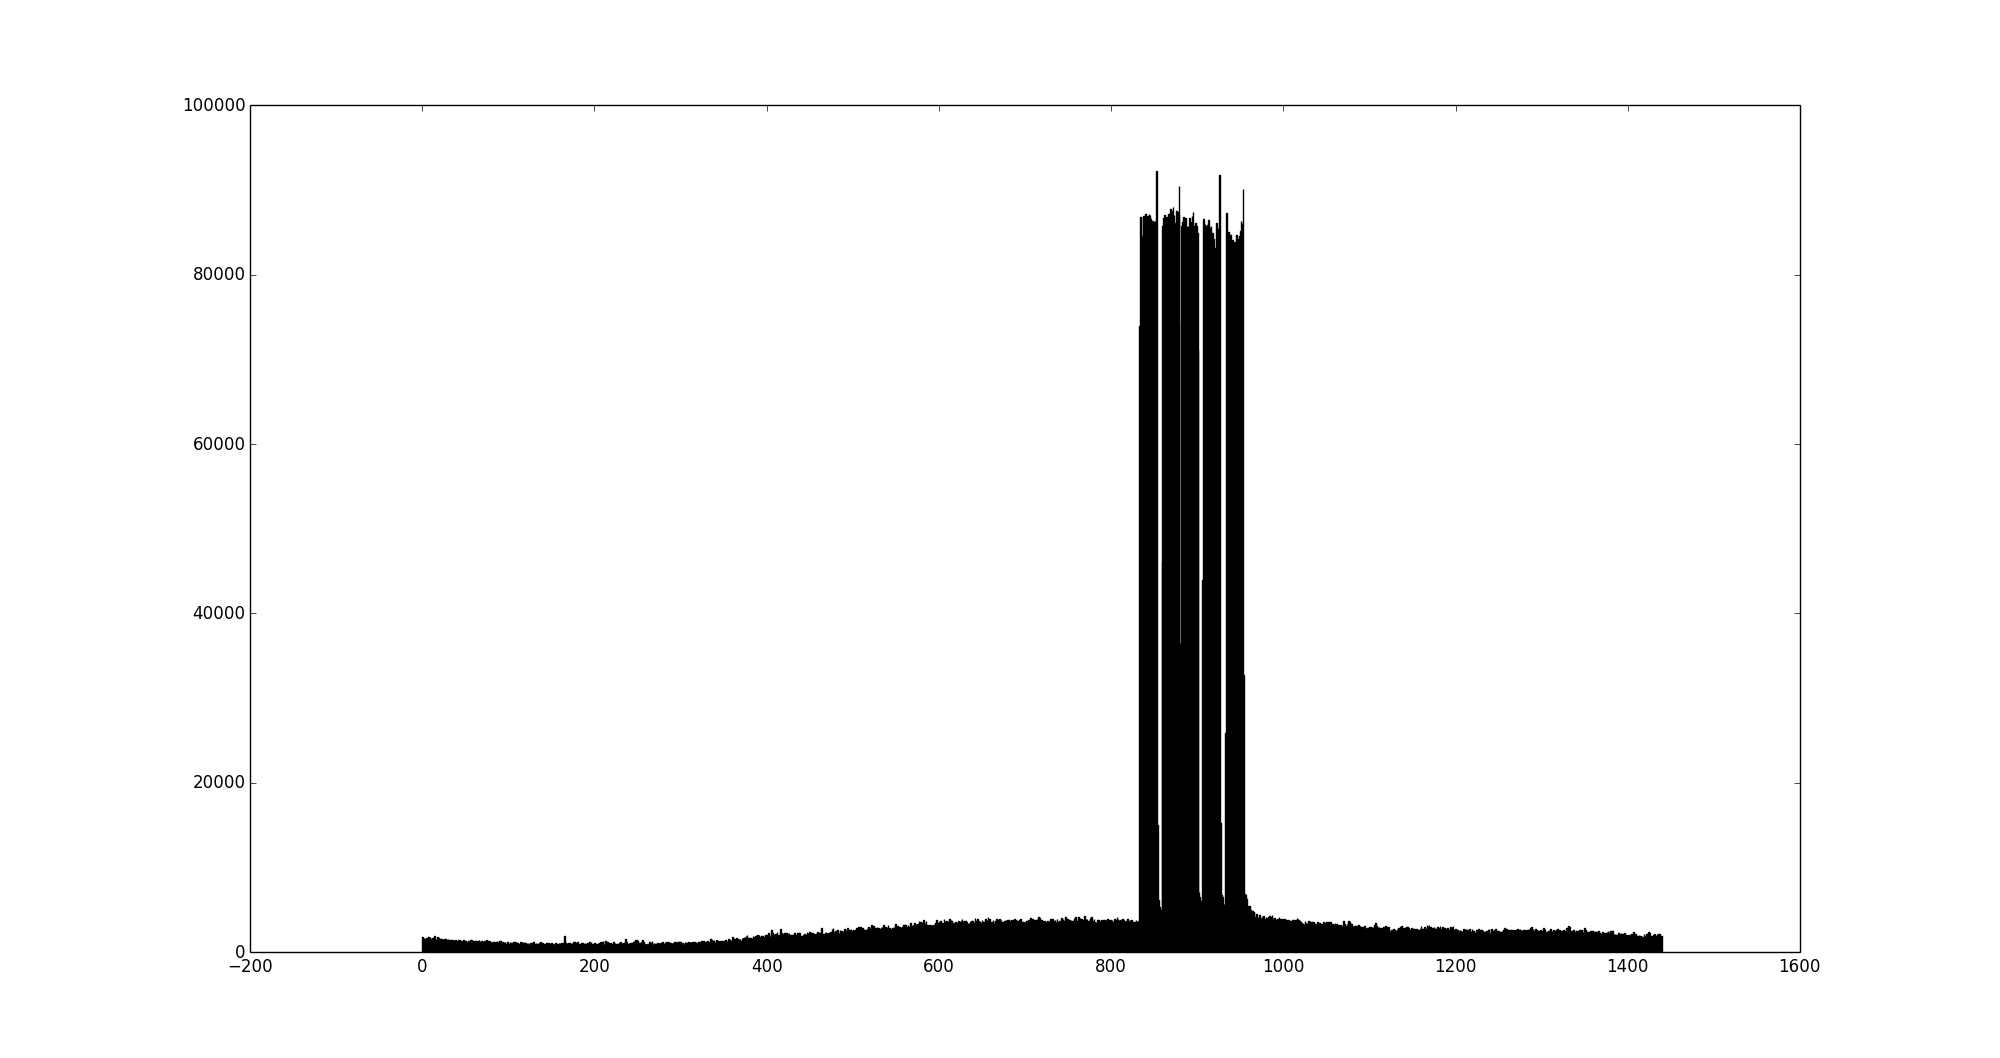
\includegraphics[width=\textwidth]{all-activity.png}
  \caption{Linjer i loggen pr. minut}
  \label{fig:ddos-all-activity}
\end{figure}

\begin{figure}[h!]
  \centering
  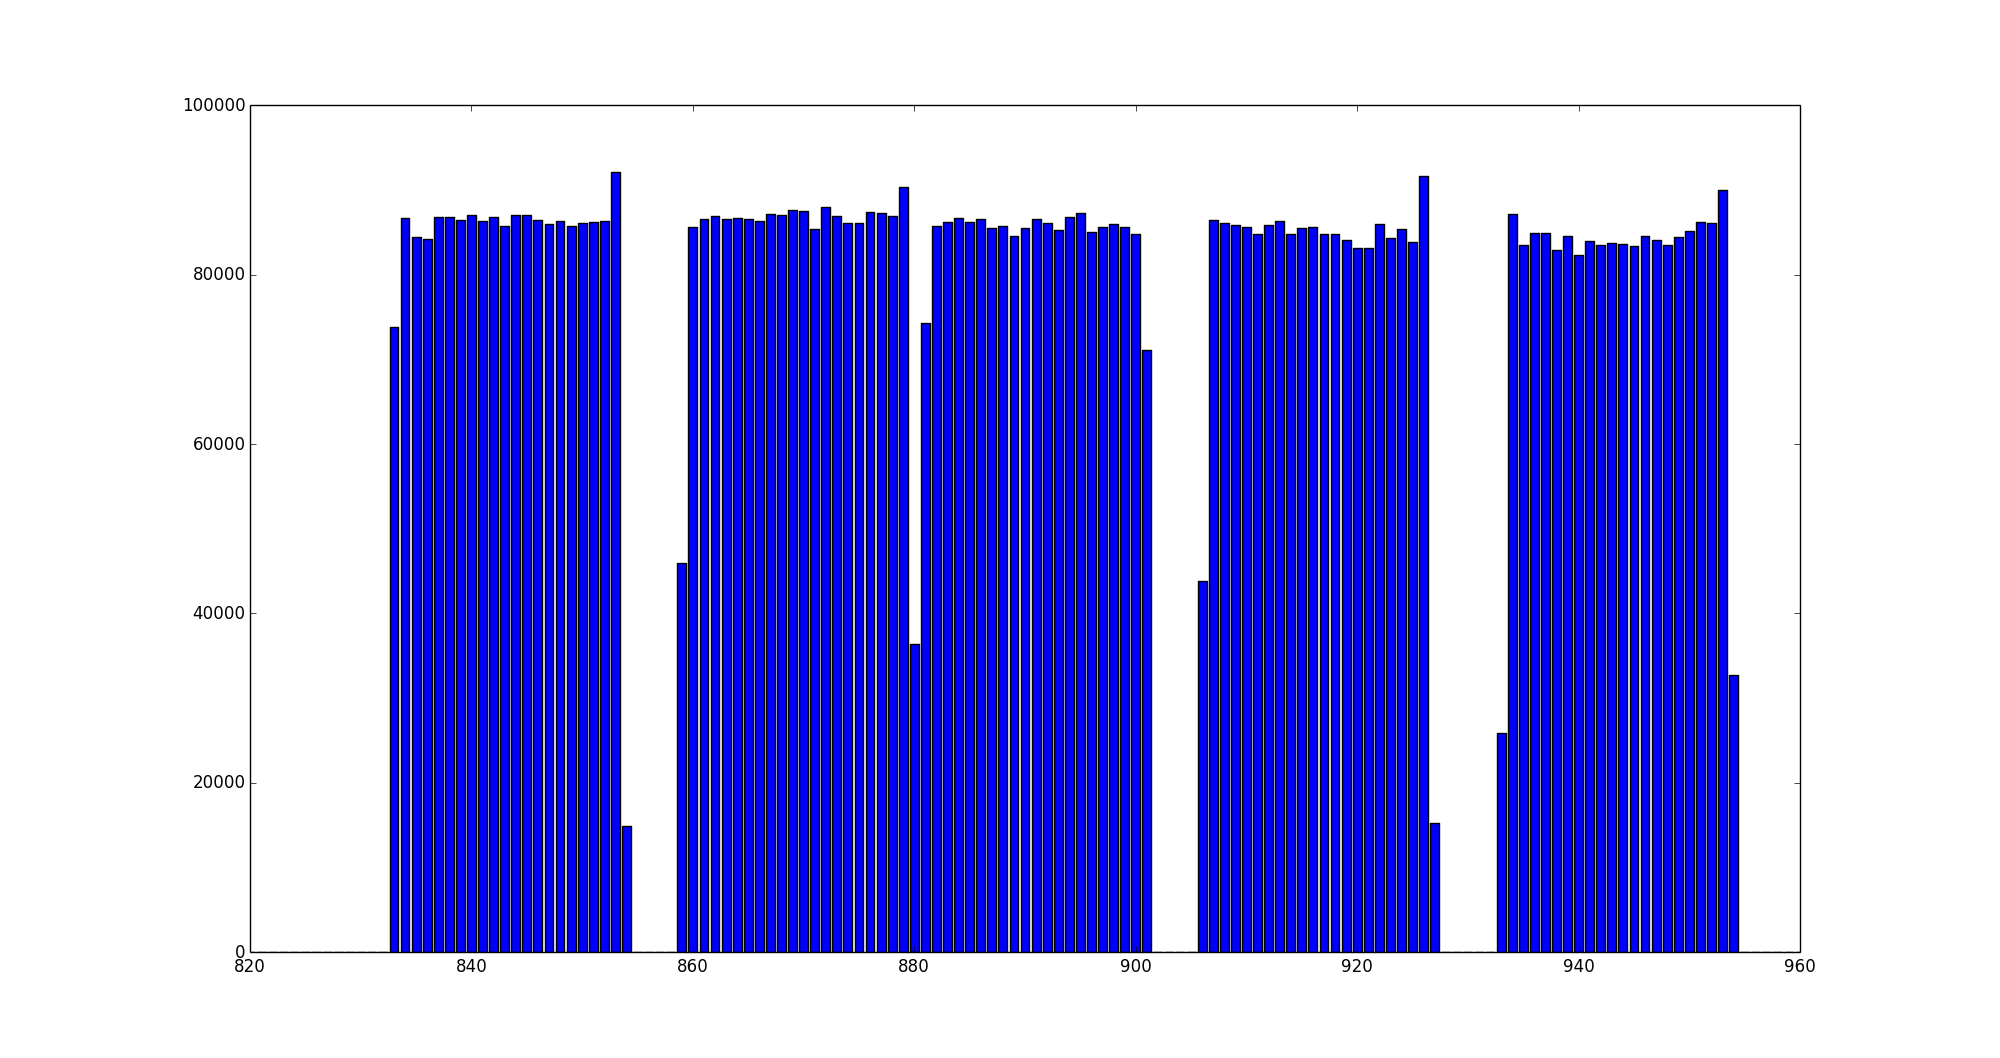
\includegraphics[width=\textwidth]{udp-activity.png}
  \caption{linjer i loggen der nævner udp pr. minut (startende fra minut 833 = kl. 13.53)}
  \label{fig:ddos-udp-activity}
\end{figure}

\begin{figure}[h!]
  \centering
  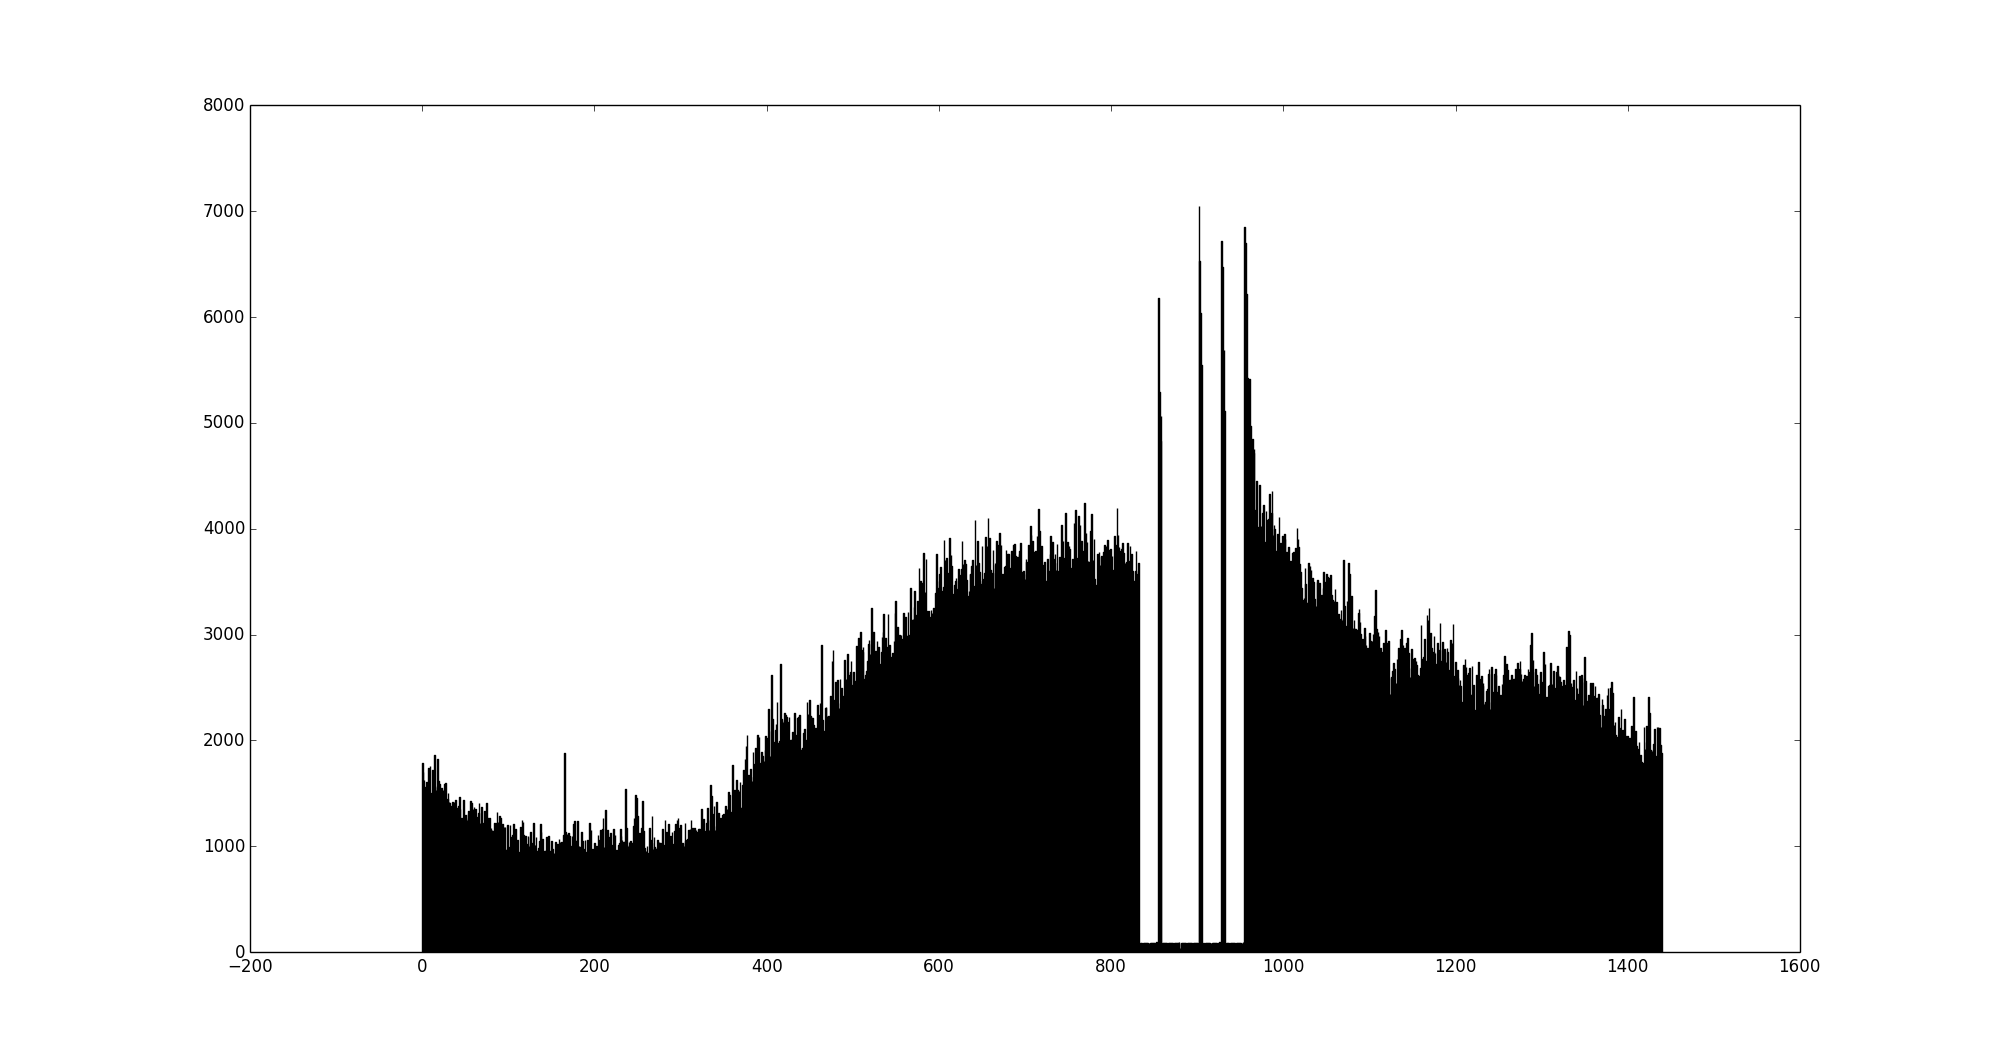
\includegraphics[width=\textwidth]{non-udp-activity.png}
  \caption{Linjer i loggen med andet end UDP pr. minut}
  \label{fig:ddos-non-udp-activity}
\end{figure}

\newpage

\section{Office 365}
Vi får at vide, at BIOchem gerne vil skifte deres nuværende Office løsning ud,
så de ikke længere har en fysisk installation på hver maskine.
De vil i stedet skifte til Office 365 for, at de ikke skal sørge for at opdatere
Office pakkerne på computerne og derved undgå mulighederne for manglende patches
giver problemer.

Vi vil her komme med de ting vi mener, at vi bør have med, hvis vi skulle lave
en sikkerhedsanalyse af BIOchems Office 365 valg.

\subsection{Hvordan ser løsningen ud?}
I denne del ville vi komme ind på, hvordan selve løsningen ser ud, så vi også
selv har et overblik over, hvad det egentlig er vi arbejder med.
Her kunne vi kigge på forskellige sikkerhedsrapporter omkring systemet og
whitepapers, der evt. beskriver, hvordan systemet er bygget på.
Dette vil give os en bedre mulighed for at komme med kvalificerede bud på
evt. sikkerhedsproblemer.

\subsection{Sikkerhedsmål}
Her vil vi komme ind på, hvilke mål vi har for vores løsning. Det er vigtig,
at de er veldefineret, så vi ikke skyder over eller under målet for, hvad
vi gerne vil beskytte.

\subsection{Hvad vil vi gerne beskytte?}
I denne sektion kommer vi så ind på, hvad det er vi gerne vil beskytte.
For hvert aktiv vi beskriver vil vi også beskrive dets værdi, hvilket
kan være omkostningerne for at erstatte det, vigtigheden for virksomhedens
funktion osv.
Dette gør vi igen for at indskrænke og komme tættere på, hvilke reelle
problemstillinger vi står overfor.

\subsection{Risici}
I denne del ville vi kigge på de enkelte trusler, som vi kunne forestille os,
at der ville være i forbindelse med et skifte til Office 365 og hvordan det
kunne påvirke BIOchem.

Nogle af disse trusler kunne f.eks. være:
\begin{description}
    \item En bruger får kompromiteret sin adgang pga. et man-in-the-middle angreb.
    \item En bruger med et dårligt løsen får kompromiteret sin adgang.
    \item Microsofts backend bliver hacket og hackere får adgang til BIOchems data.
\end{description}

Disse problemstillinger ville vi så gennemgå hver for sig og komme med en
vurdering af, hvor store problemer de evt. kunne skabe for BIOchem.
Vi vil komme ind på omkostninger, hvis BIOchem løber ind i disse problemer,
samt hvor sandsynlige de er og hvad der kan gøres for at undgå disse problemer.
Vi vil også komme ind på, om der allerede er taget højde for nogle af disse ting
i det nuværende system.

Disse data vil vi så stille op i en risiko matrix, som giver et hurtigt overblik
over, hvordan de forskellige risici er placeret i forhold til hinanden, så det
er nemt at se, hvilket der bør reageres på.

\subsection{Hvilke ting bør der reageres på?}
Her vil vi komme ind på, hvilke trusler der bør reageres på. Her kan vi tage
udgangspunkt i vores risiko matrix og kigge på de risici, der ligger på den
forkerte ende af skalaen.

\subsection{Opsummering}
Til sidst vil vi komme med en opsummering af, hvad vi er kommet frem til igennem
hele rapporten.


\section{Litteraturliste}

\begin{thebibliography}{9}

\bibitem{cracking}
  \url{http://www.onlinehashcrack.com/how_to_crack_windows_passwords.php}, 21.
  maj 2014.

\bibitem{donotuse} Microsoft Developer Network,
  \url{http://msdn.microsoft.com/en-us/library/cc236715.aspx}

\bibitem{cracker1} \url{http://www.hashkiller.co.uk/ntlm-decrypter.aspx}
\bibitem{cracker2} \url{http://rainbowtables.it64.com/}

\end{thebibliography}


\end{document}
